\documentclass[tikz]{standalone}
\usepackage{tikz-feynhand}
\usepackage{feynmf}
% bubble diagram
\begin{document}
% bubble diagram
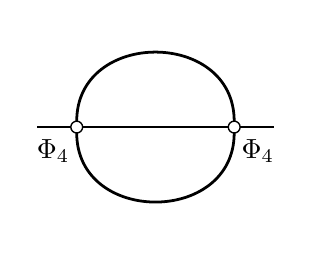
\begin{tikzpicture}
\begin{feynhand}
\vertex[ringdot] (a) at (0,0){}; 
\vertex[ringdot] (b) at (2,0){}; 
\vertex (c) at (2.5,0);\vertex (d) at (-0.5,0); % 両端
\propag[plain,line width = 1pt] (b) to (c);
\propag[plain,line width = 1pt] (d) to (a); %両端
\propag[plain,line width = 1pt] (a) to [in=90, out=90, looseness=1.5] (b);     % bubble部分
\propag[plain,line width = 1pt] (a) to [in=270, out=270, looseness=1.5] (b); % bubble部分
\propag[plain,line width = 1pt] (a) to  (b); % bubble部分

\node at (-0.3,-0.3) {$\Phi_4$};
\node at (2.3,-0.3) {$\Phi_4$};
\end{feynhand}
\end{tikzpicture}
\end{document}

